\chapter{Validación y Resultados}\label{cap:Validacion}
%Se deben incluir tantos cap\'{\i}tulos como se requieran; sin embargo, se recomienda que la tesis  o trabajo de investigaci\'{o}n tenga un m\'{\i}nimo 3 cap\'{\i}tulos y m\'{a}ximo de 6 cap\'{\i}tulos (incluyendo las conclusiones).\\

%\renewcommand{\tablename}{\textbf{Código}}
\section{Traducción a Código}
En esta Sección se muestran porciones del modelo ejecutable que se programa en C++ \citep{ISO:2017:IIIa}. Se elije este lenguaje porque la \textit{Stardard Template Library} (STL) tiene facilidades que permiten hacer explícita la consistencia del código con el esquema preconceptual. Se emula una base de datos a partir de arreglos globales que almacenan cada concepto, y, las claves foráneas que se generan entre conceptos se traducen como punteros. \\

A continuación se muestra, a modo de ejemplo, las traducciones de algunos conceptos, funciones, o porciones del EP a código C++ para verificar la consistencia del código con el modelo ejecutable. Primero, se definen los elementos que conforman las condiciones iniciales, y, la base de datos que se emula, es decir, los arreglos que contienen los conceptos que se instancian en la ejecución de las relaciones dinámicas del EP. Posteriormente, se muestran las traducciones a código de dos conceptos clase, ``Malla'' y ``Roca'', y la traducción de la relación dinámica ``Petrofísico caracteriza Roca''. Luego, se explica la traducción del cálculo del residual en el evento ``Presión del Fluido Varía''.\\

Las condiciones iniciales, en las que se definen variables globales y constantes, se programan en un \textit{namespace} ``Global'' que agrupa todas las definiciones, tal como aparecen en la figura \ref{fig:EjInitialConditions}. El código para las condiciones iniciales se expone en la Tabla \ref{tab:InitialConditions}.\\

\begin{table}[h!]
	\centering
	\begin{tabular}{cc}
		\parbox[c]{10em}{
			\begin{tabular}[c]{@{}c@{}}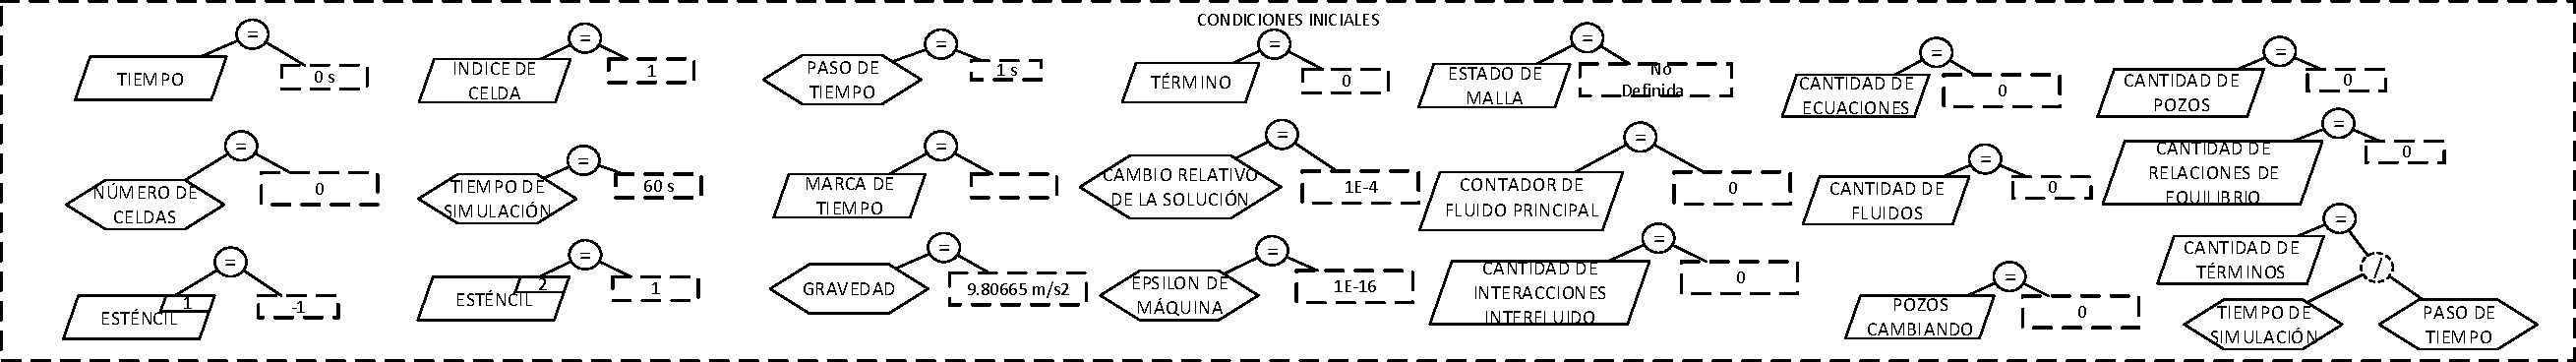
\includegraphics[width=3in]{Fig/EjInitialConditions.pdf}\\ Ver figura \ref{fig:EjInitialConditions}.\end{tabular}
			%
			%\caption[Elementos para la representación de Software Científico.]{Elementos para la representación de Software Científico. \citep{JCalle,norena2018det}.} \label{fig:RockTranslation}
		}
		&
		\begin{tiny}
			\begin{lstlisting}
			namespace Initial_Conditions{
			
			std::string timestamp="";
			double mytime=0;
			double simulationtime = 86400;
			double timedelta=1;
			int wells_quantity=0;
			int term=0;
			int fluids_quantity=0;
			int stencil[2] = {-1,1};
			int equilibrium_relations_quantity=0;
			int interfluid_interactions_quantity=0;
			int cells_number=0;
			int changing_wells=0;
			
			};
			
			\end{lstlisting}
		\end{tiny}
	\end{tabular}
	\caption[Traducción a código de las condiciones iniciales.]{Traducción a código de las condiciones iniciales. Los autores. \label{tab:InitialConditions}}
\end{table}

En el código de la Tabla \ref{tab:bd} se muestran los conceptos que se almacenan en arreglos, estos se iteran en diferentes funciones del código. Es importante notar que, en las precondiciones del EP se establece que sólo se define una única malla y sólo se caracteriza una única roca. Por tanto, en la base de datos que se emula, estos dos conceptos se acceden por medio de un puntero único. También se destaca que, todos los objetos que se instancian de los conceptos clase, se acceden a partir de punteros. Todos los punteros se fundamentan en la STL, que se encarga de hacer la respectiva gestión del uso de la memoria.\\

\begin{table}[h!]
	\begin{tabular}{c}
		\begin{tiny}
			\begin{lstlisting}
			
			std::vector<std::shared_ptr<Equation_Base>> equations =
			std::vector<std::shared_ptr<Equation_Base>>();
			
			std::vector<std::shared_ptr<Fluid>> characterized_fluids =
			std::vector<std::shared_ptr<Fluid>>();
			
			std::vector<std::unique_ptr<Equilibrium_Relation>> added_equilibrium_relations =
			std::vector<std::unique_ptr<Equilibrium_Relation>>();
			
			std::vector<std::unique_ptr<Interfluid_Interaction>> added_interfluid_interactions =
			std::vector<std::unique_ptr<Interfluid_Interaction>>();
			
			std::vector<std::shared_ptr<Well>> perforated_wells =
			std::vector<std::shared_ptr<Well>>();
			
			std::unique_ptr<Mesh> mymesh;
			std::unique_ptr<Rock> myrock;
			
			\end{lstlisting}
		\end{tiny}
	\end{tabular}
	\caption[Arreglos que conforman la base de datos que se emula.]{Arreglos que conforman la base de datos que se emula. Los autores. \label{tab:bd}}
\end{table}

En el código de la Tabla \ref{tab:MeshCode} se puede observar que, la conceptualización de la malla coincide con el código que se genera para la misma. La malla se propone como un conjunto de celdas. Adicionalmente, se tienen elementos como el espesor que dependen de la cantidad de celdas en cada dirección. Las celdas también se iteran, pero su arreglo correspondiente se almacena dentro del concepto malla, tal como se propone en la sección \ref{subsec:PS_Mesh}.\\

\begin{table}[h!]
	\centering
	\begin{tabular}{cc}
		\parbox[c]{5em}{
			\begin{tabular}[c]{@{}c@{}}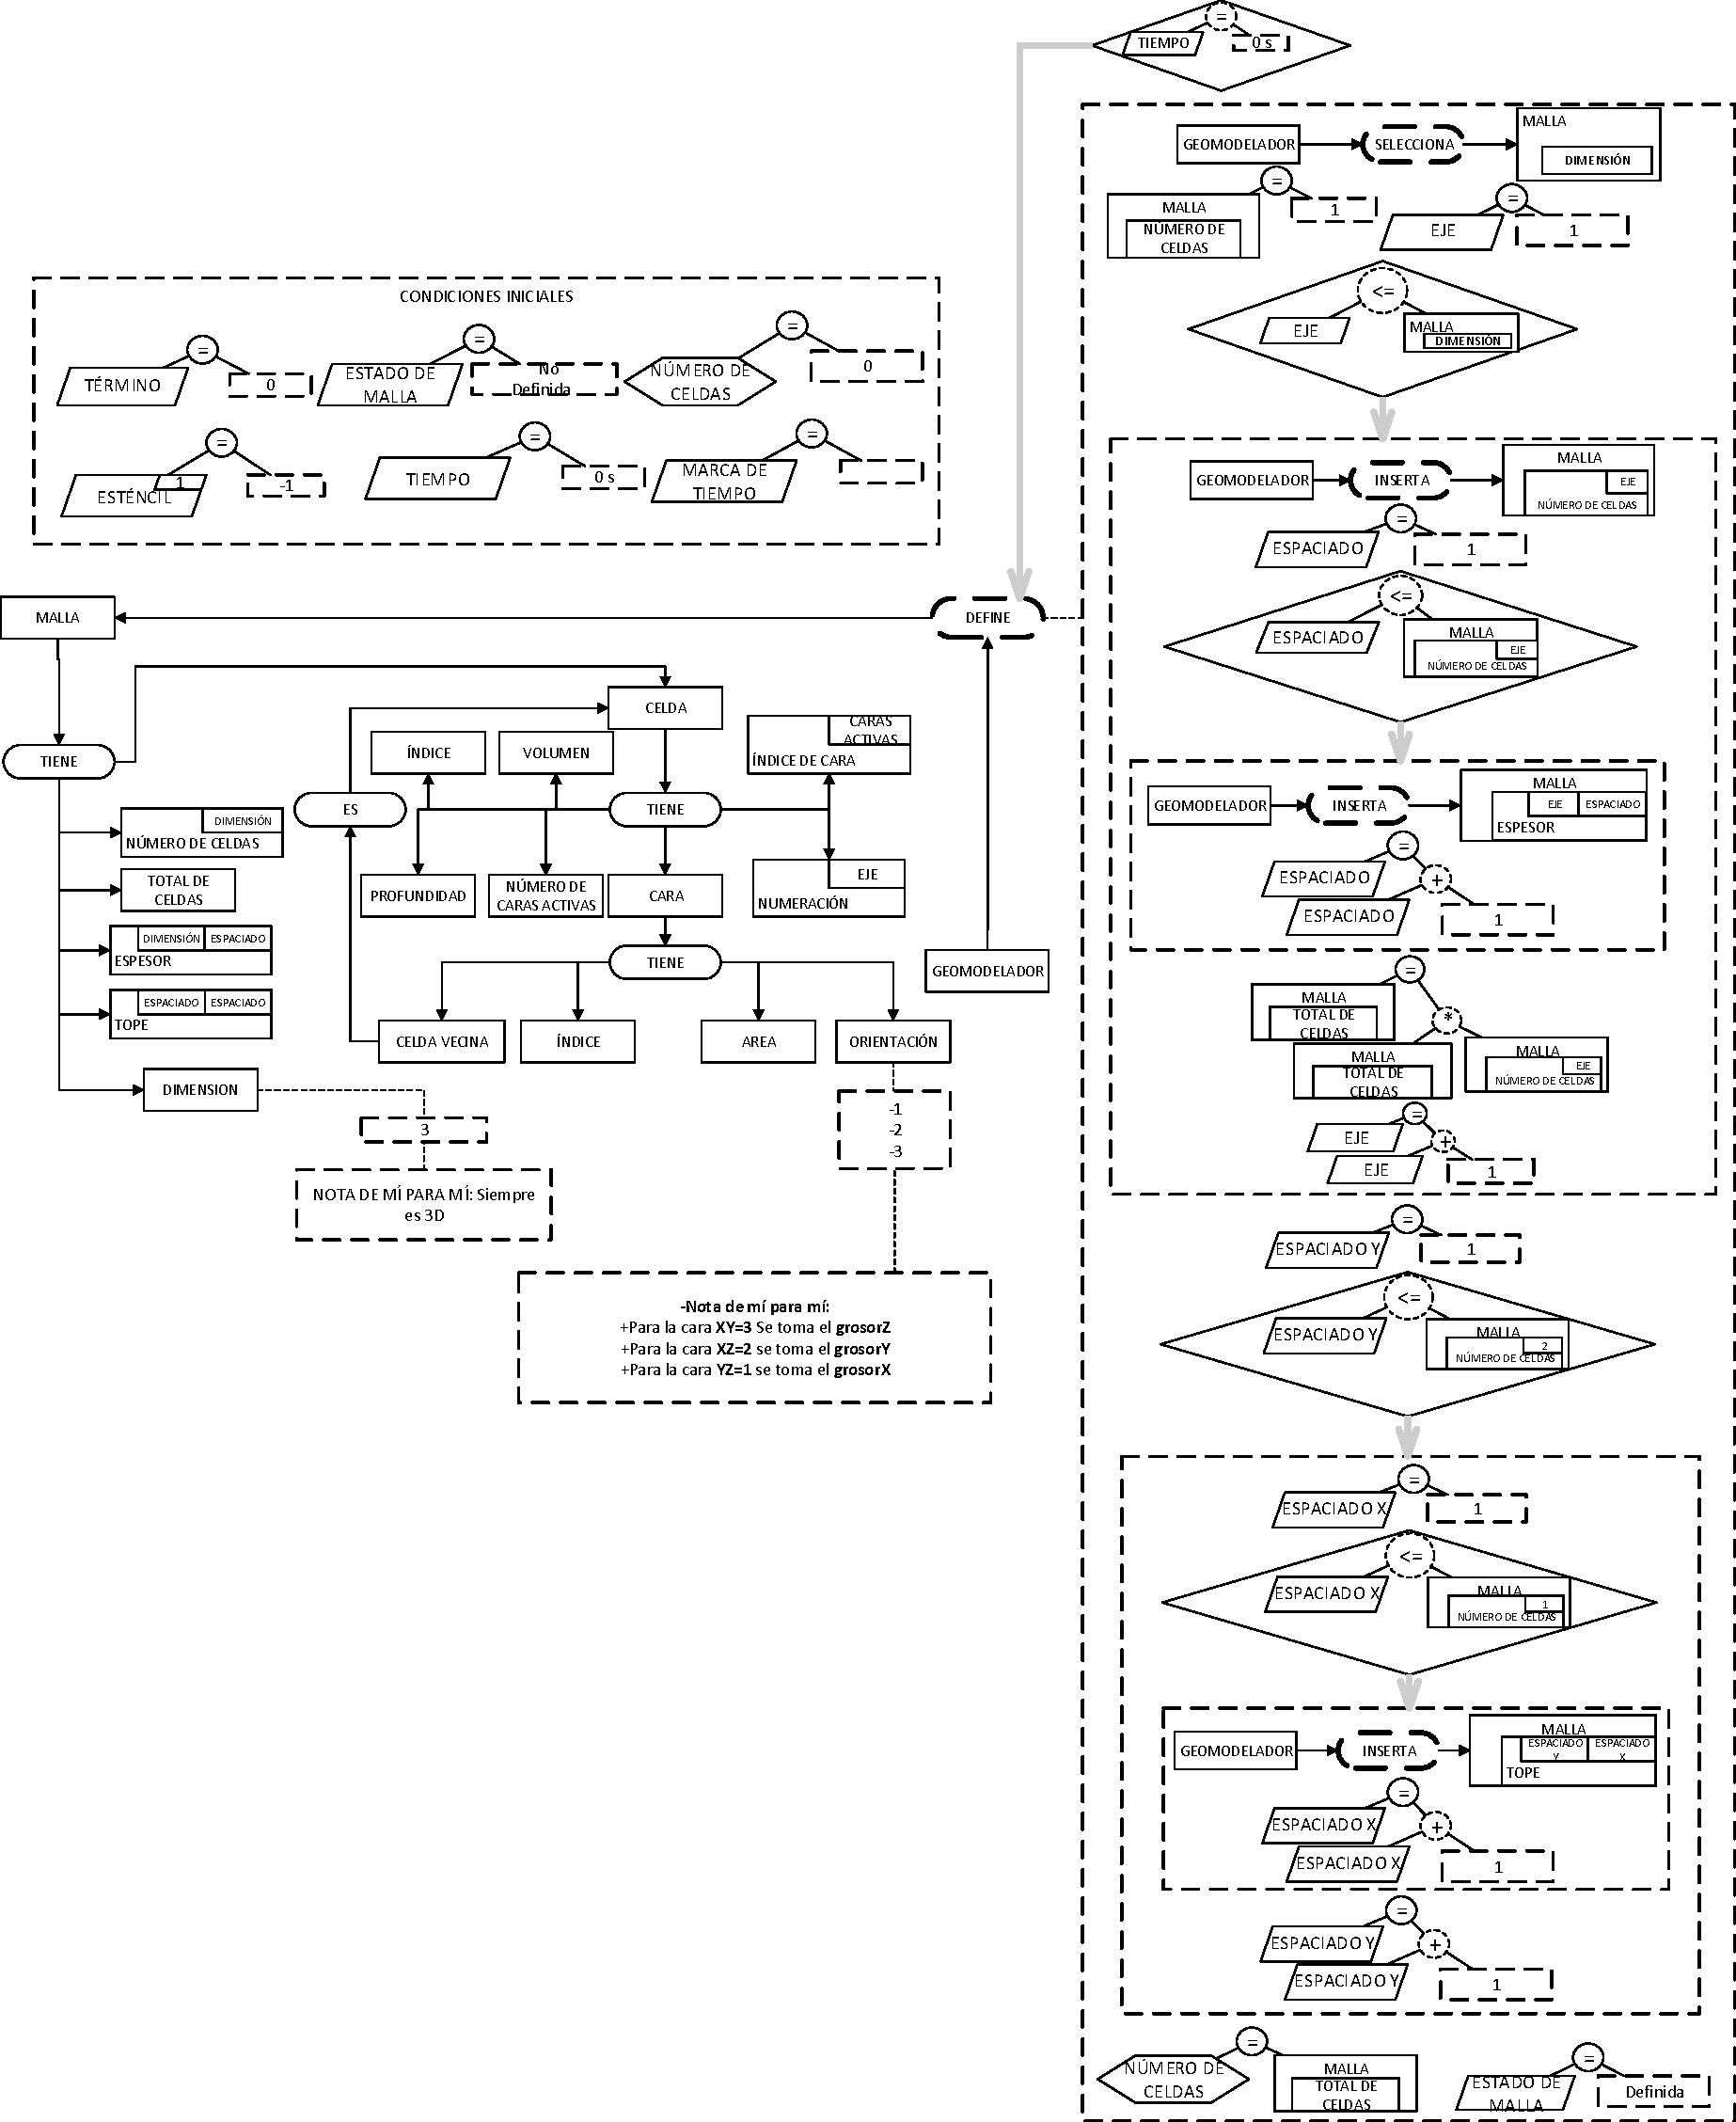
\includegraphics[width=2in]{Fig/Mesh.pdf}\\ Ver figura \ref{fig:Mesh}.\end{tabular}
			%
			%\caption[Elementos para la representación de Software Científico.]{Elementos para la representación de Software Científico. \citep{JCalle,norena2018det}.} \label{fig:RockTranslation}
		}
		&
		\begin{tiny}
			\begin{lstlisting}
			
			class Mesh{
			
			private:
			
			using Cells_t = std::vector<std::shared_ptr<Cell>>;
			int _dimension;
			std::vector<int> _cell_number = std::vector<int>(3);
			int _cell_total;
			std::vector<std::vector<double>> _thickness;
			std::vector<std::vector<double>> _top;
			int _defined=0;
			Cells_t _cells;
			
			public:
			
			using Cell_iterator = Cells_t::iterator;
			using Cell_const_iterator = Cells_t::const_iterator;
			
			Mesh();
			int getCellTotal();
			void define();
			void defineFromFile(std::ifstream& mesh_reader);
			void appear(const std::string& _timestamp, const int stencil[2]);
			
			int listCell(int posx, int posy, int posz);
			int listCell(std::vector<int> _Numeration);
			
			const std::shared_ptr<Cell>& cell(const int index) const 
			{return _cells[index];};
			
			const double& thickness(const int axis, const int spacing) const 
			{return _thickness[axis][spacing];};
			
			Cell_iterator begin() {return _cells.begin();};
			Cell_iterator end()   {return _cells.end();};
			
			Cell_const_iterator begin()  const {return _cells.begin();};
			Cell_const_iterator end()    const {return _cells.end();};
			Cell_const_iterator cbegin() const {return _cells.cbegin();};
			Cell_const_iterator cend()   const {return _cells.cend();};
			
			
			};
			
			\end{lstlisting}
		\end{tiny}
	\end{tabular}
	\caption[Traducción a código del concepto Malla.]{Traducción a código del concepto Malla. Los autores. \label{tab:MeshCode}}
\end{table}

\newpage

En el código de la Tabla \ref{tab:RockCode}, se muestra la definición de la clase Roca, que corresponde al concepto roca en el EP y se pueden notar adicionalmente, la implementación de los \textit{get} y \textit{set} para cada atributo o concepto hoja. En el código de la Tabla \ref{tab:RockCharacterizeCode} se muestra la implementación de la relación dinámica ``petrofísico caracteriza roca''. Ésta se implementa como lecturas por consola, la cuál se desarrolla de manera segura en la función \textit{myRead}. Se logra evidenciar la consistencia en los nombres de los atributos, parámetros y las variables independientes que se definen en la lectura. Adicionalmente, por las dimensiones de los casos que se simulan, se implementa una lectura equivalente usando archivos para mayor facilidad de uso.

\begin{table}[h!]
	\centering
	\begin{tabular}{cc}
		\parbox[c]{1em}{
			\begin{tabular}[c]{@{}c@{}}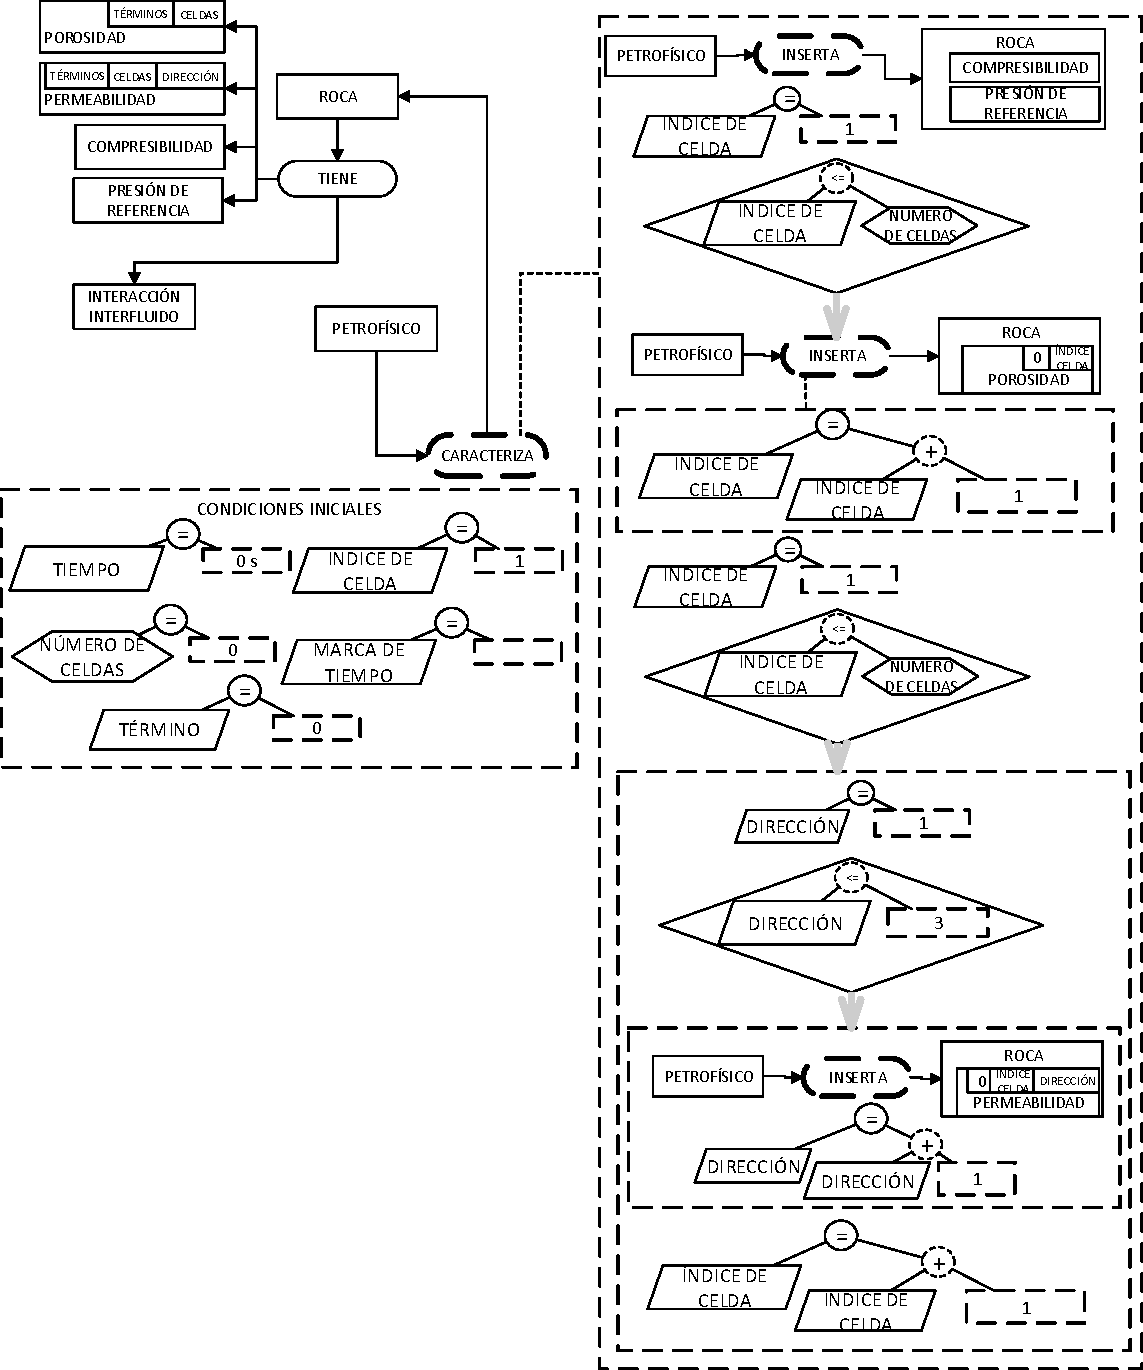
\includegraphics[width=1in]{Fig/Rock.pdf}\\ Ver figura \ref{fig:Rock}.\end{tabular}
			%
			%\caption[Elementos para la representación de Software Científico.]{Elementos para la representación de Software Científico. \citep{JCalle,norena2018det}.} \label{fig:RockTranslation}
		}
		&
		\begin{tiny}
			\begin{lstlisting}
			class Rock{
			private:
			
			double _reference_pressure;
			double _compressibility;
			std::vector<std::vector<std::vector<double>>> _absolute_permeability;   
			std::vector<std::vector<double>> _porosity;
			
			public:
			
			Rock(){};
			void characterize(const int& cells_number);
			void characterizeFromFile(std::ifstream& rock_reader,
			const int& cells_number);
			void porosity(const int term, const int cell_index,
			const double pressure);
			
			void updateProperties(const int& term);
			
			const double& porosity (const int term, const int cells_number) const {
			return _porosity[term][cells_number];
			};
			
			const std::vector<double>& absolutePermeability
			(const int term, const int cells_number) const {
			return _absolute_permeability[term][cells_number];
			};
			};
			
			\end{lstlisting}
		\end{tiny}
	\end{tabular}
	\caption[Traducción a código del concepto Roca.]{Traducción a código del concepto Roca. Los autores. \label{tab:RockCode}}
\end{table}

\begin{table}[h!]
	\centering
	\begin{tabular}{cc}
		\parbox[c]{5em}{
			\begin{tabular}[c]{@{}c@{}}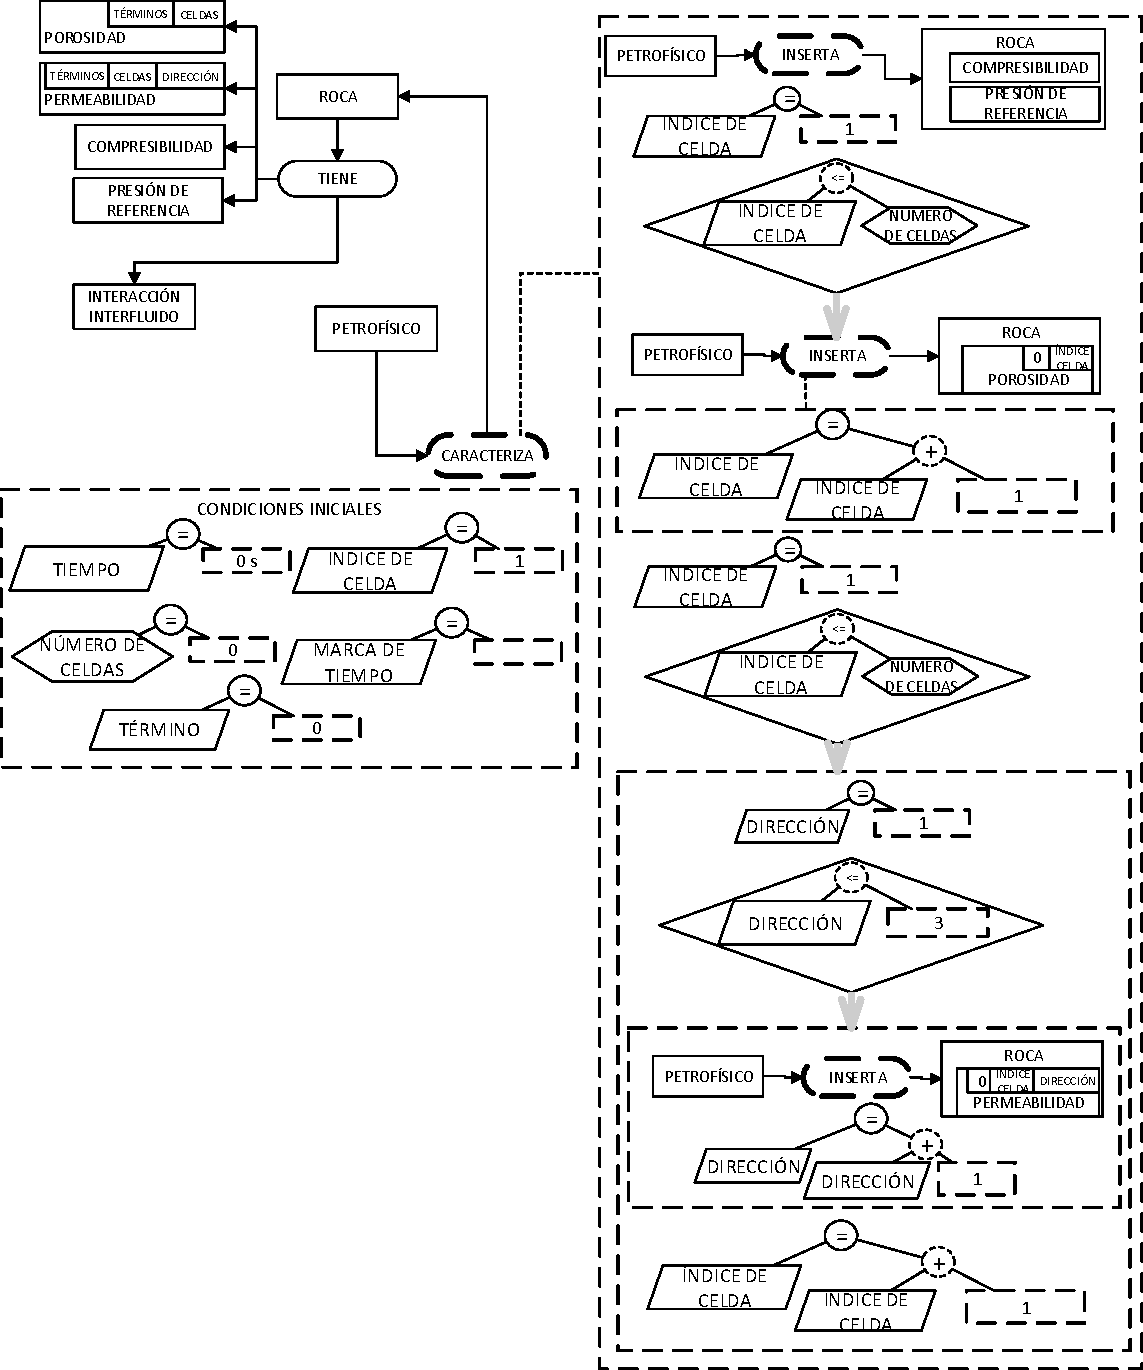
\includegraphics[width=1.5in]{Fig/Rock.pdf}\\ Ver figura \ref{fig:Rock}.\end{tabular}
			%
			%\caption[Elementos para la representación de Software Científico.]{Elementos para la representación de Software Científico. \citep{JCalle,norena2018det}.} \label{fig:RockTranslation}
		}
		&
		\begin{tiny}
			\begin{lstlisting}
			void Rock::characterize(const int& cells_number){
			
			std::ostringstream ss = std::ostringstream();
			const std::string axisnames[3]={"x", "y", "z"};
			
			_absolute_permeability = std::vector<std::vector<std::vector<double>>>
			(1,std::vector<std::vector<double>>(cells_number,std::vector<double>(3)));
			_porosity              = std::vector<std::vector<double>>(1,std::vector<double>(cells_number));
			
			myRead(std::string("Please insert rock compressibility [1/Pa]"), _compressibility,
			std::string("Please insert a valid input"));
			
			myRead(std::string("Please insert reference pressure [Pa]"), _reference_pressure,
			std::string("Please insert a valid input"));
			
			for(int cellindex=0; cellindex<cells_number; ++cellindex){
			
			ss << "Please insert initial porosity for the "<< cellindex+1 << " cell [-]";
			myRead(ss.str(), _porosity[0][cellindex], std::string("Please insert a valid input"));
			ss.str("");
			ss.clear();
			
			
			};
			for(int cellindex=0; cellindex<cells_number; ++cellindex){
			for(int direction=0; direction<3;++direction){
			ss << "Please insert initial absolute permeability for the "<< cellindex+1
			<< " cell in direction " << axisnames[direction] << " [m2]";
			myRead(ss.str(), _absolute_permeability[0][cellindex][direction],
			std::string("Please insert a valid input"));
			ss.str("");
			ss.clear();
			};
			};
			};
			
			\end{lstlisting}
		\end{tiny}
	\end{tabular}
	\caption[Traducción a código de la relación dinámica ``Petrofísico caracteriza Roca''.]{Traducción a código de la relación dinámica ``Petrofísico caracteriza Roca''. Los autores. \label{tab:RockCharacterizeCode}}
\end{table}
\newpage

En el código de la Tabla \ref{tab:ResidualCode} se evidencia cómo se logra iterar entre los conceptos. Por ejemplo para las ecuaciones, usando los vectores con los que se emula la base de datos, se logra realizar el cálculo del residual consistentemente con la representación. La operación de obtención de tipo, se desarrolla como un método interno dentro de la clase \textit{Equation\_Base}, con el fin de mantener la equivalencia casi exacta entre la representación y el código C++. Luego, la operación de asignación de tipo de ecuación, a fluido o a pozo, se convierte en una conversión de tipo o \textit{cast}.

\begin{table}[h!]
	\centering
	\begin{tabular}{cc}
		\parbox[c]{7em}{
			\begin{tabular}[c]{@{}c@{}}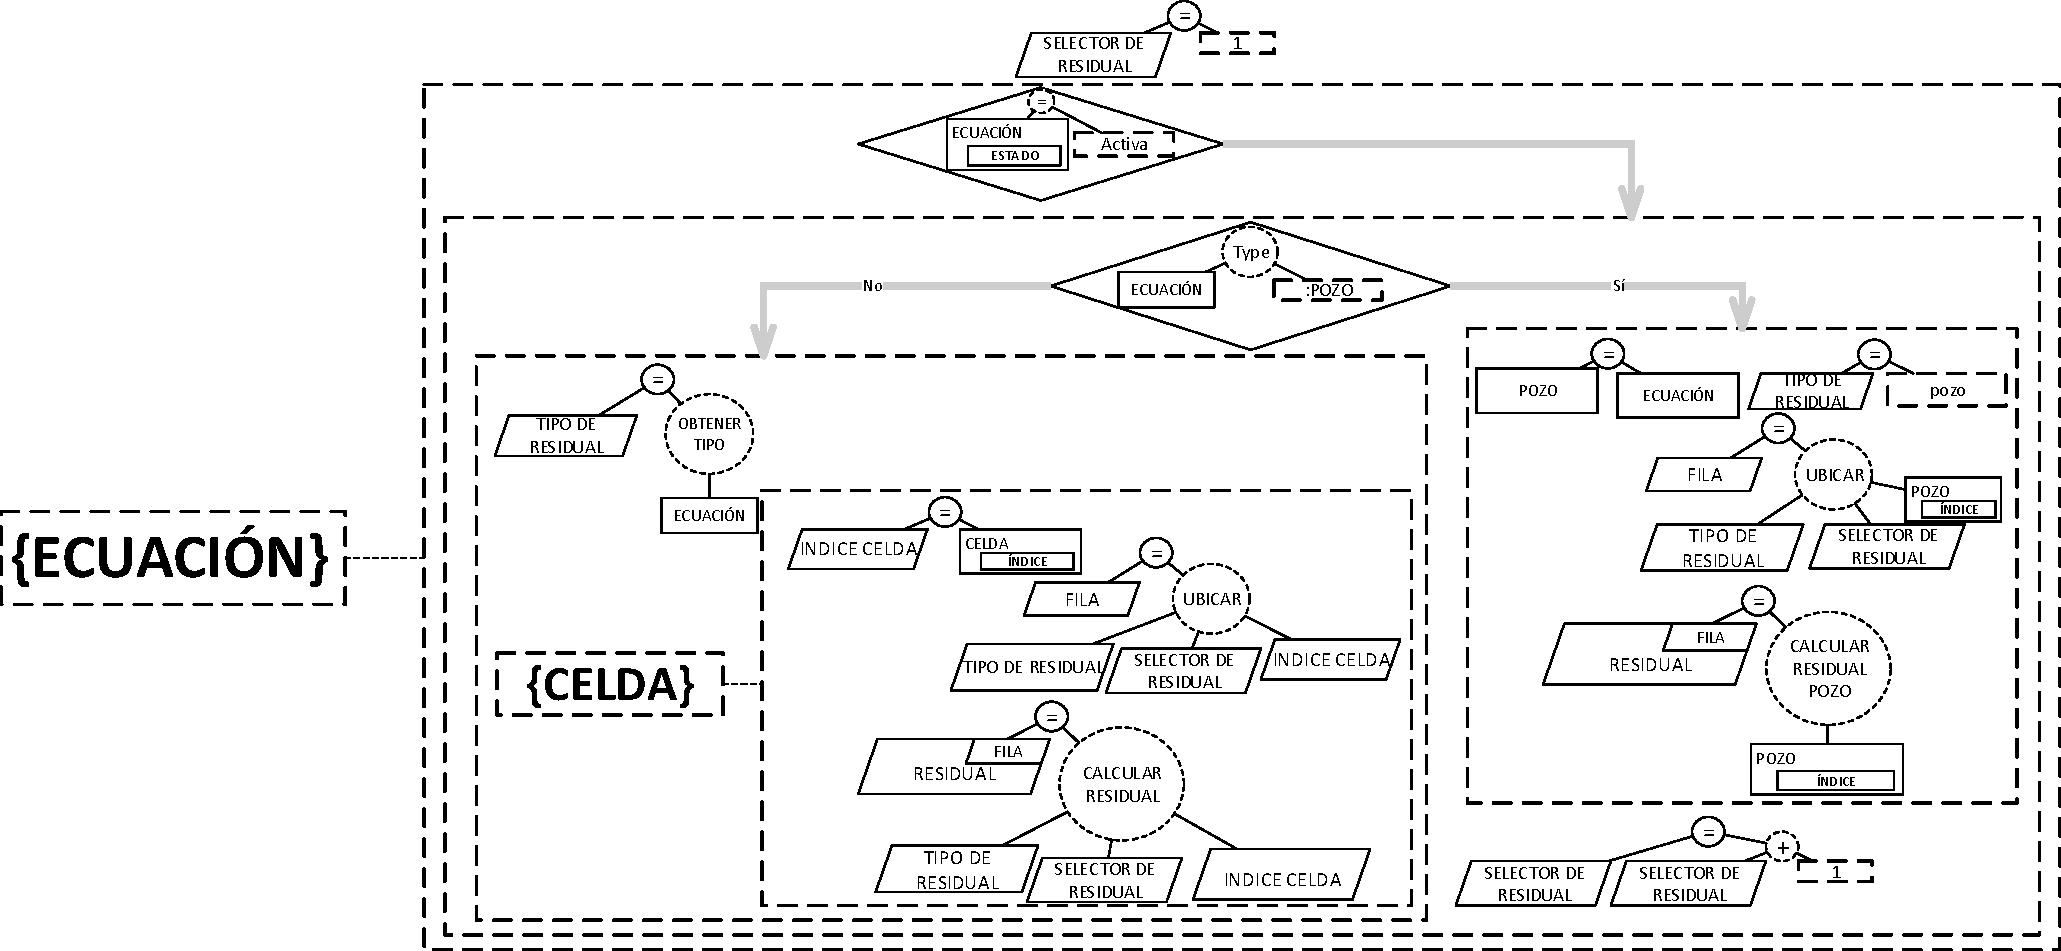
\includegraphics[width=2.5in]{Fig/Residual.pdf}\\ Ver figura \ref{fig:Residual}.\end{tabular}
			%
			%\caption[Elementos para la representación de Software Científico.]{Elementos para la representación de Software Científico. \citep{JCalle,norena2018det}.} \label{fig:RockTranslation}
		}
		&
		\begin{tiny}
			\begin{lstlisting}
			//Residual calculation
			residual_selector = 0;
			
			for(auto equation : equations){
			
			if(equation->status()){
			
			if(equation->type() == typeid(Well).name()){
			
			constexpr auto residual_type = "well";
			auto residual_well = std::dynamic_pointer_cast<Well,Equation_Base>(equation);
			
			row = locate(residual_type, residual_selector, residual_well->index());
			_residual(row) = calculateWellResidual(term, residual_well);
			
			}else{
			
			constexpr auto residual_type = "fluid";
			auto residual_fluid = std::dynamic_pointer_cast<Fluid,Equation_Base>(equation);
			
			for(auto cell = mesh.begin(); cell != mesh.end(); ++cell){
			
			cell_index = (*cell)->index();
			
			row = locate(residual_type, residual_selector, cell_index);
			
			_residual(row) = 
			calculateResidual(term,*residual_fluid, mesh, *cell, rock, wells);
			
			};
			};
			
			++residual_selector;
			
			};
			};
			
			\end{lstlisting}
		\end{tiny}
	\end{tabular}
	\caption[Traducción a código del cálculo de residual en el evento ``Presión del Fluido Varía''.]{Traducción a código del cálculo de residual en el evento ``Presión del Fluido Varía''. Los autores. \label{tab:ResidualCode}}
\end{table}


\section{Caso de Literatura}
En esta Sección se pretende validar el modelo ejecutable que se realiza a partir del esquema preconceptual. Con éste propósito, se plantea un caso que se toma de \cite{jamal2006petroleum}. El cual, consiste en una simulación de un yacimiento lineal (1D) de cinco celdas con un solo fluido y un pozo productor en la cuarta celda, como se muestra en la Figura \ref{fig:Abou-Kassem} \citep{jamal2006petroleum}. Con este, se espera validar el transporte de un fluido y las pérdidas de presión por pozos.\\

El caso de estudio de \cite{jamal2006petroleum} consta de dos procesos principales, uno de pérdidas a caudal fijo, y el otro, cuando la celda perforada para el pozo alcanza la ``presión de abandono''. En este, se cambia la condición operativa del pozo para mantener la presión fija a esa presión de abandono. En la Figura \ref{fig:ConstantQ} se reportan los resultados de la simulación durante la etapa de producción a caudal constante, y en la Figura \ref{fig:ConstantP} se reportan los resultados de la simulación durante la etapa de producción a presión constante.
\begin{figure}[h!]
	\centering
	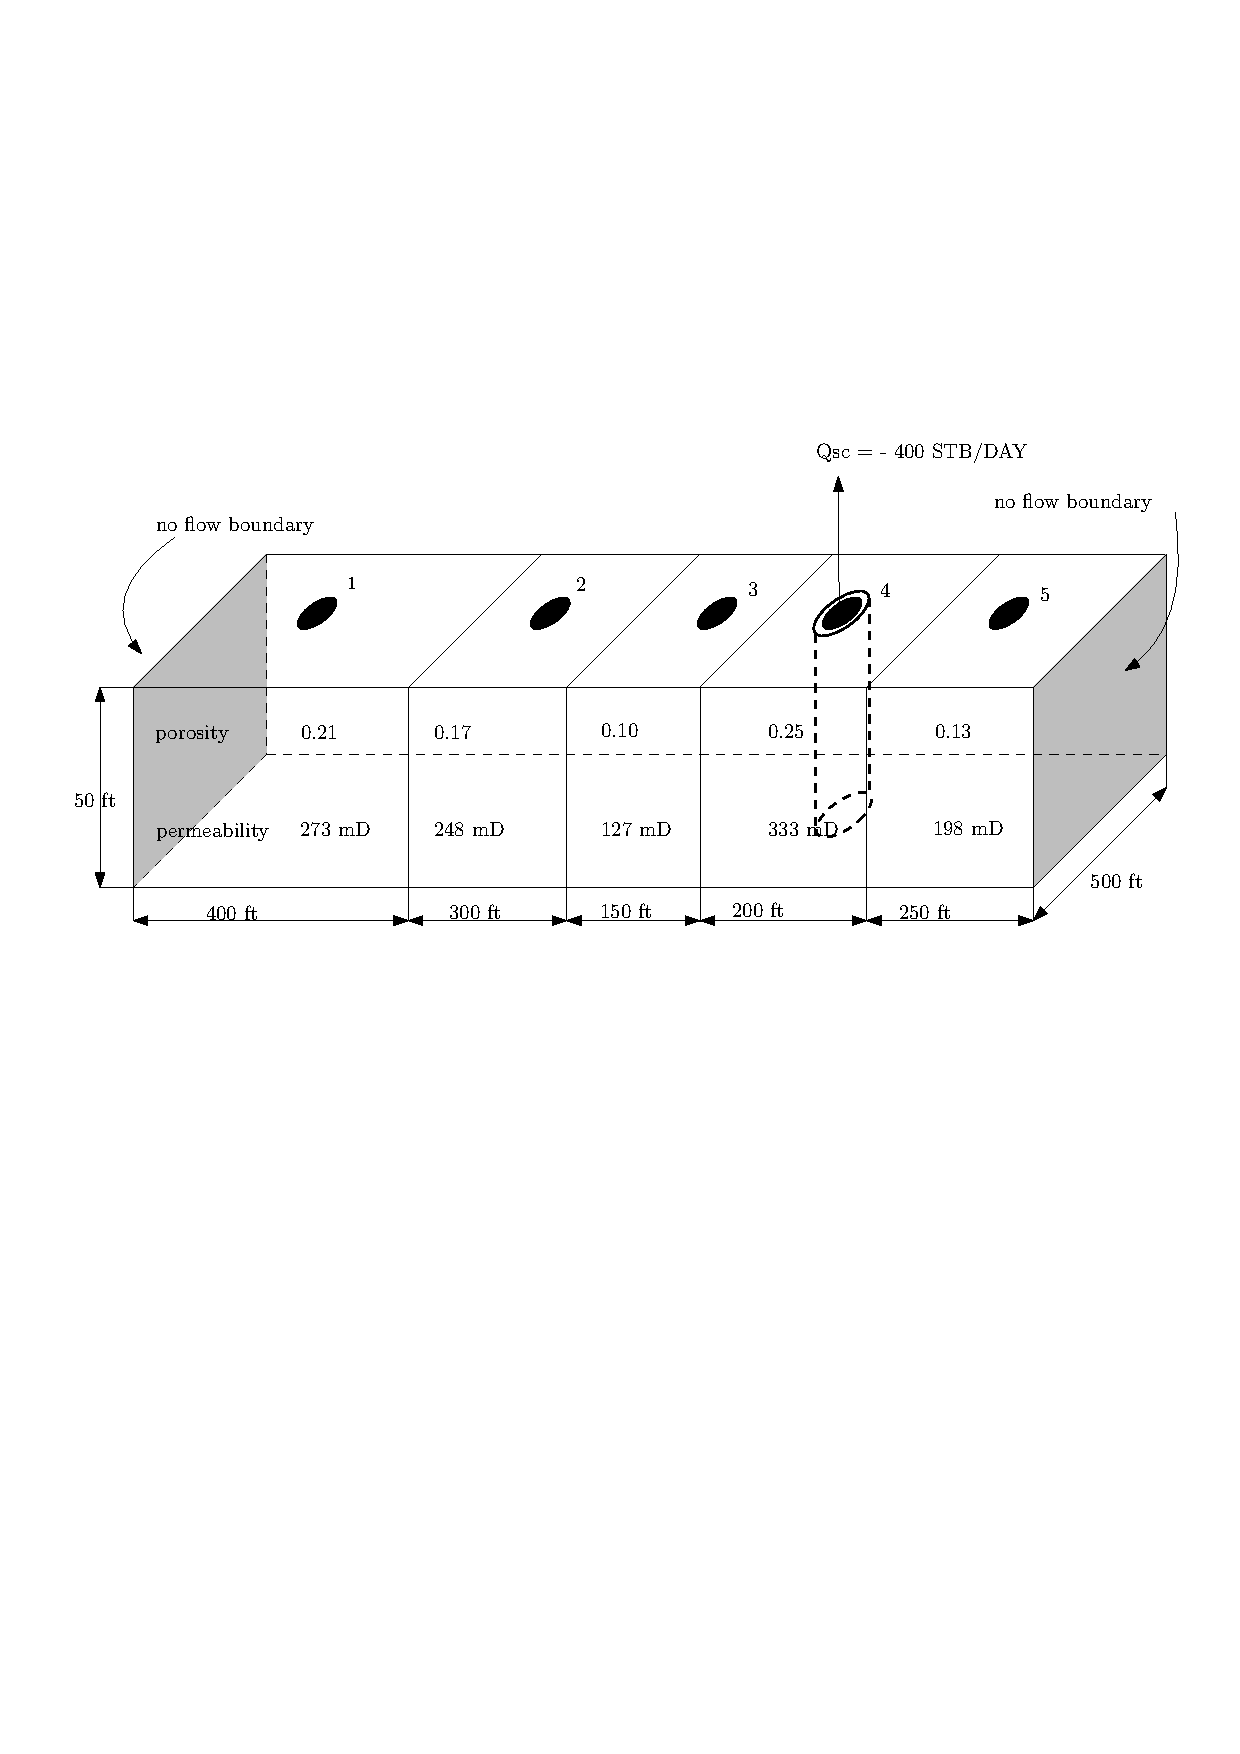
\includegraphics[width=0.9\textwidth]{Fig/casoasis.pdf}
	\caption{Representación gráfica del caso proporcionado por \cite{jamal2006petroleum}.}
	\label{fig:Abou-Kassem}
\end{figure}



\begin{figure}[h!]
	\centering
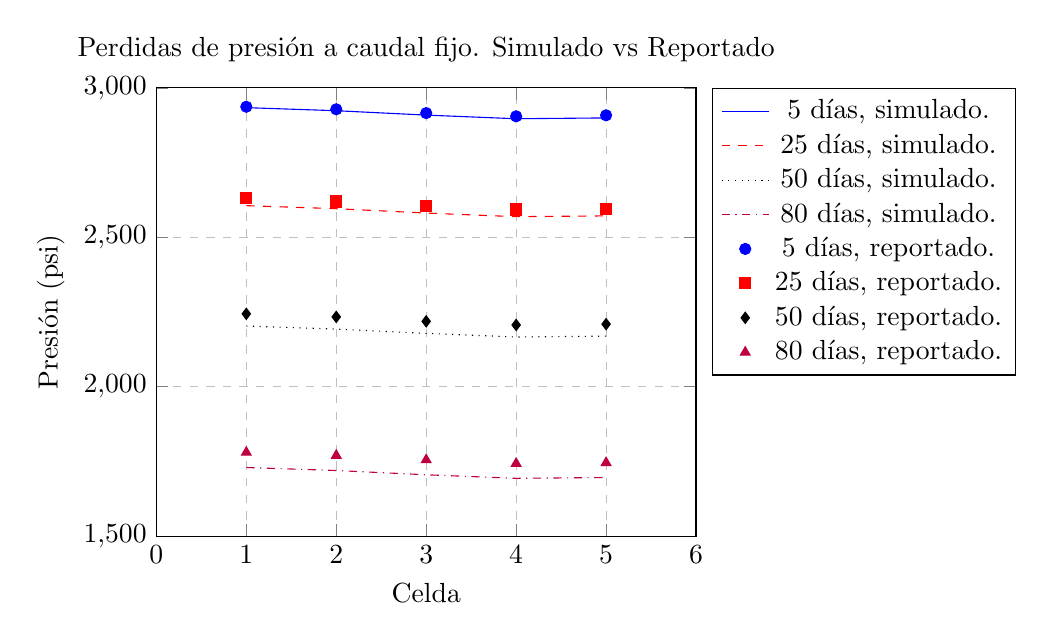
\begin{tikzpicture}
\begin{axis}[
title={Perdidas de presión a caudal fijo. Simulado vs Reportado},
xlabel={Celda},
ylabel={Presión (psi)},
xmin=0, xmax=6,
ymin=1500, ymax=3000,
legend pos=outer north east ,
ymajorgrids=true,
xmajorgrids=true,
%semilogxaxis=true,
grid style=dashed,
]

\addplot[color=blue]
coordinates{
	(1,2933.8141602)
	(2,2923.5889812)
	(3,2908.882128)
	(4,2896.698936)
	(5,2899.4836656)
	
};
\addlegendentry{5 días, simulado.}

\addplot[dashed, color=red]
coordinates{
	(1,2605.9267536)
	(2,2595.745086)
	(3,2581.1107518)
	(4,2569.0000788)
	(5,2571.741297)
	
};
\addlegendentry{25 días, simulado.}

\addplot[dotted,color=black]
coordinates{
	(1,2203.1127162)
	(2,2193.0180714)
	(3,2178.5287752)
	(4,2166.5196288)
	(5,2169.2463432)
	
};
\addlegendentry{50 días, simulado.}

\addplot[dashdotted,color=purple]
coordinates{
	(1,1729.7812032)
	(2,1719.8025888)
	(3,1705.4728344)
	(4,1693.6087260)
	(5,1696.3064328)
};
\addlegendentry{80 días, simulado.}

\addplot[only marks, mark options={draw=blue,fill=blue,}]
coordinates{
	(1,2936.80)
	(2,2928.38)
	(3,2915.68)
	(4,2904.88)
	(5,2908.18)
	
	
};
\addlegendentry{5 días, reportado.}
\addplot[only marks, mark=square*, mark options={draw=red,fill=red,}]
coordinates{
	(1,2630.34)
	(2,2620.06)
	(3,2605.28)
	(4,2593.04)
	(5,2595.81)
	
	
};
\addlegendentry{25 días, reportado.}
\addplot[only marks, mark=diamond*, mark options={draw=black,fill=black,}]
coordinates{
	(1,2243.97)
	(2,2233.68)
	(3,2218.9)
	(4,2206.66)
	(5,2209.43)
	
	
};
\addlegendentry{50 días, reportado.}
\addplot[only marks, mark=triangle*, mark options={draw=purple,fill=purple,}]
coordinates{
	
	(1,1780.3100)
	(2,1770.0200)
	(3,1755.2400)
	(4,1743.0000)
	(5,1745.7700)
	
	
};
\addlegendentry{80 días, reportado.}
\end{axis}
\end{tikzpicture}
\caption{Comparativo datos simulados contra caso de estudio de \cite{jamal2006petroleum}. Caudal constante.}
\label{fig:ConstantQ}
\end{figure}{}

Las condiciones iniciales de presión para el yacimiento son de $3000$ $psia$ para todas las celdas y el pozo se establece a una condición operativa de caudal fijo a $400$ $STB/D$. Se puede ver como en los primeros 80 días, va decayendo la presión hasta alcanzar la presión de abandono. Se encuentran diferencias entre los resultados simulados y los reportados por \cite{jamal2006petroleum} menores a $50$ $psia$. Éstas se deben, a que las ecuaciones que se implementan en el modelo ejecutable, son diferentes a las que se presentan en \cite{jamal2006petroleum}.

\begin{figure}[h!]
	\centering
	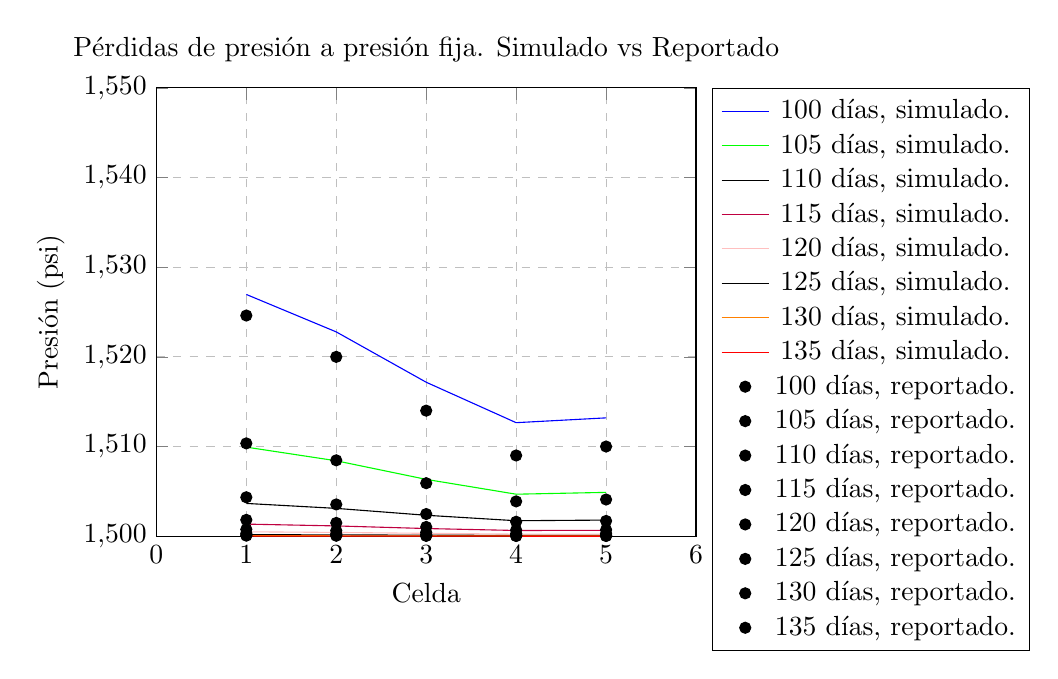
\begin{tikzpicture}
	\begin{axis}[
	title={Pérdidas de presión a presión fija. Simulado vs Reportado},
	xlabel={Celda},
	ylabel={Presión (psi)},
	xmin=0, xmax=6,
	ymin=1500, ymax=1550,
	legend pos=outer north east ,
	ymajorgrids=true,
	xmajorgrids=true,
	%semilogxaxis=true,
	grid style=dashed,
	]
	
	\addplot[color=blue]
	coordinates{
		(1,	1526.960064 )
		(2,	1522.7829696)
		(3,	1517.169999)
		(4,	1512.6593172)
		(5,	1513.1959578)
	};
	\addlegendentry{100 días, simulado.}
	
	\addplot[color=green]
	coordinates{
		(1,	1509.9326028)
		(2,	1508.4097038)
		(3,	1506.3356604)
		(4,	1504.6822272)
		(5,	1504.8852804)
	};
	\addlegendentry{105 días, simulado.}
	
	\addplot[color=black]
	coordinates{
		(1,	1503.6524574)
		(2,	1503.101313)
		(3,	1502.3326116)
		(4,	1501.723452)
		(5,	1501.795971)
	};
	\addlegendentry{110 días, simulado.}
	
	\addplot[color=purple]
	coordinates{
		(1,	1501.3463532)
		(2,	1501.1433)
		(3,	1500.853224)
		(4,	1500.635667)
		(5,	1500.6501708)
	};
	\addlegendentry{115 días, simulado.}
	
	\addplot[color=pink]
	coordinates{
		(1,	1500.490629)
		(2,	1500.41811)
		(3,	1500.3165834)
		(4,	1500.2295606)
		(5,	1500.2295606)
	};
	\addlegendentry{120 días, simulado.}
	
	
	\addplot[]
	coordinates{
		(1,	1500.1715454)
		(2,	1500.1425378)
		(3,	1500.1135302)
		(4,	1500.0845226)
		(5,	1500.0845226)
	};
	\addlegendentry{125 días, simulado.}
	
	\addplot[color=orange]
	coordinates{
		(1,	1500.055515)
		(2,	1500.0410112)
		(3,	1500.0265074)
		(4,	1500.0265074)
		(5,	1500.0265074)
	};
	\addlegendentry{130 días, simulado.}
	
	
	\addplot[red]
	coordinates{
		(1,	1500.0120036)
		(2,	1500.0120036)
		(3,	1500.0120036)
		(4,	1499.9974998)
		(5,	1499.9974998)
	};
	\addlegendentry{135 días, simulado.}
	
	
	\addplot[only marks]
	coordinates{
		(1,	1524.61)
		(2,	1520)
		(3,	1514)
		(4,	1509 )
		(5,	1510)
		
	};
	\addlegendentry{100 días, reportado. }
	
	\addplot[only marks]
	coordinates{
		(1,	1510.35)
		(2,	1508.46)
		(3,	1505.91)
		(4,	1503.88)
		(5,	1504.09)
		
	};
	\addlegendentry{105 días, reportado.}
	
	\addplot[only marks]
	coordinates{
		(1,	1504.34)
		(2,	1503.54)
		(3,	1502.47)
		(4,	1501.61)
		(5,	1501.7)
	};
	\addlegendentry{110 días, reportado. }
	
	\addplot[only marks]
	coordinates{
		(1,	1501.82)
		(2,	1501.48)
		(3,	1501.03)
		(4,	1500.68)
		(5,	1500.71)
	};
	\addlegendentry{115 días, reportado.}
	
	\addplot[only marks]
	coordinates{
		(1,	1500.76)
		(2,	1500.62)
		(3,	1500.43)
		(4,	1500.28)
		(5,	1500.3)
	};
	\addlegendentry{120 días, reportado.}
	
	
	\addplot[only marks]
	coordinates{
		(1,	1500.32)
		(2,	1500.26)
		(3,	1500.18)
		(4,	1500.12)
		(5,	1500.12)
	};
	\addlegendentry{125 días, reportado.}
	
	\addplot[only marks]
	coordinates{
		(1,	1500.13)
		(2,	1500.11)
		(3,	1500.08)
		(4,	1500.05)
		(5,	1500.05)
	};
	\addlegendentry{130 días, reportado.}
	
	
	\addplot[only marks]
	coordinates{
		(1	,1500.06)
		(2	,1500.05)
		(3	,1500.03)
		(4	,1500.02)
		(5	,1500.02)
	};
	\addlegendentry{135 días, reportado.}
	
	\end{axis}
	\end{tikzpicture}
	\caption{Comparativo datos simulados contra caso de estudio de \cite{jamal2006petroleum}. Presión constante.}
	\label{fig:ConstantP}
\end{figure}{}

En la etapa de producción a presión constante se logra observar como la presión del sistema decae hasta que se estabiliza completamente a la presión de abandono. En esta etapa se siguen observando diferencias de alrededor de $10$ $psia$. Con este comportamiento se logra validar el modelo ejecutable para la simulación de casos de producción por flujo natural. Para ejecutar casos en los que se involucren más fenómenos físicos, se requiere un control numérico adicional que no se contempla en el desarrollo de esta Tesis de Maestría.
